% ------------------------------------------------------------------------------
% TYPO3 CMS 8 LTS - What's New - Chapter "Deprecated Functions" (Dutch Version)
%
% @author	Michael Schams <schams.net>
% @license	Creative Commons BY-NC-SA 3.0
% @link		http://typo3.org/download/release-notes/whats-new/
% @language	English
% ------------------------------------------------------------------------------
% LTXE-CHAPTER-UID:		3f842373-9262b8d3-f9c8de76-cf29ce17
% LTXE-CHAPTER-NAME:	Deprecated Functions
% ------------------------------------------------------------------------------

\section{Verouderde/verwijderde functies}
\begin{frame}[fragile]
	\frametitle{Verouderde/verwijderde functies}

	\begin{center}\huge{\color{typo3darkgrey}\textbf{Verouderde/verwijderde functies}}\end{center}
	\begin{center}\large{\textit{}}\end{center}

\end{frame}

% ------------------------------------------------------------------------------
% LTXE-SLIDE-START
% LTXE-SLIDE-UID:		e3e5dbcf-02e1c080-d9ea7eea-a580c5f1
% LTXE-SLIDE-ORIGIN:	d4c8c340-33163839-2ae654ee-9c6834da English
% LTXE-SLIDE-TITLE:		Miscellaneous (#72337, #75150 and #73794)
% ------------------------------------------------------------------------------

\begin{frame}[fragile]
	\frametitle{Verouderde/verwijderde functies}
	\framesubtitle{Diversen}

	\begin{itemize}

		\item De volgende configuratieopties zijn verwijderd:

			\begin{itemize}
				\item \texttt{\$TYPO3\_CONF\_VARS['SYS']['t3lib\_cs\_utils']}
				\item \texttt{\$TYPO3\_CONF\_VARS['SYS']['t3lib\_cs\_convMethod']}
			\end{itemize}

			\small
				(functionaliteit wordt nu automatisch gedetecteerd en \texttt{mbstring} wordt
				standaard gebruikt indien beschikbaar)
			\normalsize

		\item De verouderde TypoScript-optie \texttt{page.includeJSlibs} is
			verwijderd. Gebruik in plaats hiervan de TypoScript-optie \texttt{page.includeJSLibs}
			(hoofdletter "L")

		\item De TypoScript-optie \texttt{config.renderCharset}, die werd gebruikt
			als tekenset voor interne conversies is verwijderd

	\end{itemize}

\end{frame}

% ------------------------------------------------------------------------------
% LTXE-SLIDE-START
% LTXE-SLIDE-UID:		82f7e930-45df84b0-147de9d7-d5523f20
% LTXE-SLIDE-ORIGIN:	dfff0a4a-601e8cb2-abb7af47-f9861736 English
% LTXE-SLIDE-TITLE:		#70056: Curl and HttpRequest removed (1)
% ------------------------------------------------------------------------------

\begin{frame}[fragile]
	\frametitle{Verouderde/verwijderde functies}
	\framesubtitle{Http-gerelateerde functies en HttpRequest klasse verwijderd (1)}

	\begin{itemize}

		\item De volgende PHP-klassen zijn \textbf{verwijderd}:

			\begin{itemize}
				\item \small\texttt{
					TYPO3\textbackslash
					CMS\textbackslash
					Core\textbackslash
					Http\textbackslash
					HttpRequest}\normalsize
				\item \small\texttt{
					TYPO3\textbackslash
					CMS\textbackslash
					Core\textbackslash
					Http\textbackslash
					Observer\textbackslash
					Download}\normalsize
			\end{itemize}

		\item De volgende opties zijn \textbf{hernoemd}:

			\begin{itemize}

				\item
					\small
						oud:\tabto{1cm}\texttt{\$TYPO3\_CONF\_VARS[HTTP][userAgent]}\newline
						nieuw:\tabto{1cm}\texttt{\$TYPO3\_CONF\_VARS[HTTP][headers][User-Agent]}

				\item
					\small
						oud:\tabto{1cm}\texttt{\$TYPO3\_CONF\_VARS[HTTP][protocol\_version]}\newline
						nieuw:\tabto{1cm}\texttt{\$TYPO3\_CONF\_VARS[HTTP][version]}

			\end{itemize}

	\end{itemize}

\end{frame}

% ------------------------------------------------------------------------------
% LTXE-SLIDE-START
% LTXE-SLIDE-UID:		745eec95-e99fc934-b30fcd58-e6405a43
% LTXE-SLIDE-ORIGIN:	ed21f1c2-5d947af5-9d35c427-05dfcf48 English
% LTXE-SLIDE-TITLE:		#70056: Curl and HttpRequest removed (2)
% ------------------------------------------------------------------------------

\begin{frame}[fragile]
	\frametitle{Verouderde/verwijderde functies}
	\framesubtitle{Http-gerelateerde functies en HttpRequest klasse verwijderd (2)}

	\begin{itemize}

		\item Alle proxy-gerelateerde opties zijn verenigd in\newline
			\small\texttt{\$TYPO3\_CONF\_VARS[HTTP][proxy]}\normalsize

		\item Alle opties voor doorverwijzingen
			(\small
				\texttt{HTTP/follow\_redirects},
				\texttt{HTTP/max\_redirects},
				\texttt{HTTP/strict\_redirects}\normalsize)
			zijn verenigd in
			\small
				\texttt{\$TYPO3\_CONF\_VARS[HTTP][allow\_redirects]}
			\normalsize

		\item Alle opties voor SSL private sleutels
			(\small
				\texttt{HTTP/ssl\_local\_cert},
				\texttt{HTTP/ssl\_passphrase}\normalsize)
			zijn samengevoegd in
			\small
				\texttt{\$TYPO3\_CONF\_VARS[HTTP][ssl\_key]}
			\normalsize

		\item Alle opties om SSL peers te verifiëren zijn samengevoegd in
			\small
				\texttt{\$TYPO3\_CONF\_VARS[HTTP][verify]}
			\normalsize

	\end{itemize}

\end{frame}

% ------------------------------------------------------------------------------
% LTXE-SLIDE-START
% LTXE-SLIDE-UID:		205063d6-50836498-3647e24f-983376a1
% LTXE-SLIDE-ORIGIN:	ab377e1e-884fa3e4-74a17b45-77aa66c0 English
% LTXE-SLIDE-TITLE:		[ExtJS Removal 1] #78521: Drop unused JavaScript from backend.js
% ------------------------------------------------------------------------------
\begin{frame}[fragile]
	\frametitle{Verouderde/verwijderde functies}
	\framesubtitle{Verwijderen ExtJS (1)}

	\begin{itemize}
		\item Als onderdeel van het verwijderen van ExtJS zijn de volgende JavaScript functies verwijderd
		 	uit de het hoofdframe van de backend (gedefinieerd in het bestand \texttt{backend.js})

		\begin{itemize}
			\item \texttt{TYPO3.\_instances}
			\item \texttt{TYPO3.addInstance}
			\item \texttt{TYPO3.getInstance}
			\item \texttt{TYPO3.helpers.split}
		\end{itemize}

	\end{itemize}

\end{frame}
% ------------------------------------------------------------------------------
% LTXE-SLIDE-START
% LTXE-SLIDE-UID:		40a76009-c8ef2793-00e65d35-d92e9405
% LTXE-SLIDE-ORIGIN:	58f2f5e1-778a1dff-969667d4-aa4c3e7b English
% LTXE-SLIDE-TITLE:		[ExtJS Removal 2] #78468: Remove ExtDirect from EXT:workspaces
% ------------------------------------------------------------------------------
\begin{frame}[fragile]
	\frametitle{Verouderde/verwijderde functies}
	\framesubtitle{Verwijderen ExtJS (2)}

	\begin{itemize}
		\item Nieuwe klasse
			\texttt{TYPO3\textbackslash
				CMS\textbackslash
				Workspaces\textbackslash
				Controller\textbackslash
				AjaxDispatcher}
			vervangt de ExtDirect router functionaliteit in \texttt{EXT:workspaces}

		\item De volgende klassen zijn verplaatst:

		\begin{itemize}
			\item \smaller\texttt{Classes/ExtDirect/AbstractHandler.php}\newline
				is nu: \texttt{Classes/Controller/Remote/AbstractHandler.php}\normalsize

			\item \smaller\texttt{Classes/ExtDirect/ActionHandler.php}\newline
				is nu: \texttt{Classes/Controller/Remote/ActionHandler.php}\normalsize

			\item \smaller\texttt{Classes/ExtDirect/MassActionHandler.php}\newline
				is nu: \texttt{Classes/Controller/Remote/MassActionHandler.php}\normalsize

			\item \smaller\texttt{Classes/ExtDirect/ExtDirectServer.php}\newline
				is nu: \texttt{Classes/Controller/Remote/RemoteServer.php}\normalsize

		\end{itemize}

	\end{itemize}

\end{frame}
% ------------------------------------------------------------------------------
% LTXE-SLIDE-START
% LTXE-SLIDE-UID:		26c7bac6-7e278402-f7bc0051-ffdfbf44
% LTXE-SLIDE-ORIGIN:	877e457d-ab15dfaa-85e46a57-335dc6a3 English
% LTXE-SLIDE-TITLE:		#78244: TYPO3_DB and Prepared Statement classes are deprecated
% ------------------------------------------------------------------------------
\begin{frame}[fragile]
	\frametitle{Deprecated/Removed Fasunctions}
	\framesubtitle{Classes \texttt{DatabaseConnection} and \texttt{PreparedStatement}}

	\begin{itemize}
		\item The following classes have been marked as \textit{deprecated}:
			\begin{itemize}
				\item \texttt{TYPO3\textbackslash
						CMS\textbackslash
						Core\textbackslash
						Database\textbackslash
						DatabaseConnection}
				\item \texttt{TYPO3\textbackslash
						CMS\textbackslash
						Core\textbackslash
						Database\textbackslash
						PreparedStatement}
			\end{itemize}
		\item Use Doctrine DBAL in TYPO3 v8 LTS instead\newline
				(\texttt{ConnectionPool} and \texttt{QueryBuilder} classes)
		\item These two classes will be removed in TYPO3 v9
	\end{itemize}

\end{frame}


% ------------------------------------------------------------------------------
% LTXE-SLIDE-START
% LTXE-SLIDE-UID:		357bd345-db584aac-e61f459c-a6047e96
% LTXE-SLIDE-ORIGIN:	70f29777-68968704-618a9b16-3bf2eea2 English
% LTXE-SLIDE-TITLE:		#78522 and #78525: JavaScript settings under TYPO3.configuration
% ------------------------------------------------------------------------------
\begin{frame}[fragile]
	\frametitle{Verouderde/verwijderde functies}
	\framesubtitle{JavaScript settings under \texttt{TYPO3.configuration}}

	\begin{itemize}
		\item The following JavaScript settings have been removed:

		\begin{itemize}
			\item \texttt{TYPO3.configuration.debugInWindow}
			\item \texttt{TYPO3.configuration.moduleMenuWidth}
			\item \texttt{TYPO3.configuration.topBarHeight}
		\end{itemize}

		\item These options were not used by the TYPO3 core anyway

	\end{itemize}

\end{frame}


% ------------------------------------------------------------------------------
% LTXE-SLIDE-START
% LTXE-SLIDE-UID:		0857cbff-8b01ade3-8fbe4d89-a505cf4b
% LTXE-SLIDE-ORIGIN:	7e836e1e-3132a797-0f3a0c68-88037011 English
% LTXE-SLIDE-TITLE:		#78581: FlexFormTools public properties dropped
% ------------------------------------------------------------------------------
\begin{frame}[fragile]
	\frametitle{Verouderde/verwijderde functies}
	\framesubtitle{Publieke eigenschappen van \texttt{FlexFormTools}}

	\begin{itemize}
		\item Twee publieke eigenschappen zijn verdwenen uit de klasse
			\texttt{TYPO3\textbackslash
				CMS\textbackslash
				Core\textbackslash
				Configuration\textbackslash
				FlexForm\textbackslash
				FlexFormTools}:

		\begin{itemize}
			\item \texttt{public \$traverseFlexFormXMLData\_DS = array();}
			\item \texttt{public \$traverseFlexFormXMLData\_Data = array();}
		\end{itemize}

		\item Het gebruik hiervan resulteert nu in een waarschuwing

	\end{itemize}

\end{frame}




% ------------------------------------------------------------------------------
% LTXE-SLIDE-START
% LTXE-SLIDE-UID:		16109dd4-2883c5a0-2122ea56-1b2e764e
% LTXE-SLIDE-ORIGIN:	82f525e3-eddc6639-96053da3-bc74d15b English
% LTXE-SLIDE-TITLE:		#78217: frameset and frame
% ------------------------------------------------------------------------------
\begin{frame}[fragile]
	\frametitle{Verouderde/verwijderde functies}
	\framesubtitle{Frameset en frame}

	\begin{itemize}
		\item \texttt{frameset} en \texttt{frame} zijn niet meer ondersteund in HTML5
		\item De volgende TypoScript objecten zijn gemarkeerd als \textit{verouderd}:

			\begin{itemize}
				\item \texttt{frameset}
				\item \texttt{frame}
			\end{itemize}

		\item De volgende TypoScript opties zijn gemarkeerd als \textit{verouderd}:

			\begin{itemize}
				\item \texttt{config.frameReloadIfNotInFrameset}
				\item \texttt{config.doctype = xhtml\_frames}
				\item \texttt{config.xhtmlDoctype = xhtml\_frames}
				\item \texttt{frameSet} \tabto{1.8cm}\textit{(en de opties)}
				\item \texttt{FRAME} \tabto{1.8cm}\textit{(en de opties)}
				\item \texttt{FRAMESET} \tabto{1.8cm}\textit{(en de opties)}
			\end{itemize}

	\end{itemize}

\end{frame}

% ------------------------------------------------------------------------------
% LTXE-SLIDE-START
% LTXE-SLIDE-UID:		8641ca19-de42f1b1-452081c2-149d85b7
% LTXE-SLIDE-ORIGIN:	1b162dfa-75daabe7-fa50f9d2-a6be83d3 English
% LTXE-SLIDE-TITLE:		!Breaking: #77460 - Extbase query cache removed
% LTXE-SLIDE-REFERENCE:	!Breaking-77460-ExtbaseQueryCacheRemoved.rst
% ------------------------------------------------------------------------------
\begin{frame}[fragile]
	\frametitle{Verouderde/verwijderde functies}
	\framesubtitle{Extbase Query Cache verwijderd}

	\begin{itemize}

		\item De op PHP gebaseerde query-cache-functionaliteit in de Extbase persistentielaag is verwijderd

		\item De volgende publieke methodes in de Extbase persistentielaag zijn verwijderd:

			\begin{itemize}
				\item \small\texttt{Typo3DbBackend->quoteTextValueCallback()}\normalsize
				\item \small\texttt{Typo3DbBackend->injectCacheManager()}\normalsize
				\item Interface definitie in \small\texttt{QuerySettingsInterface->getUseQueryCache}\normalsize
			\end{itemize}

		\item De bijbehorende cacheconfiguratie heeft geen effect meer:\newline
			\smaller
				\texttt{\$TYPO3\_CONF\_VARS[SYS][cache][cacheConfigurations]}\newline
				\tabto{0.4cm}\texttt{[extbase\_typo3dbbackend\_queries]}
			\normalsize

	\end{itemize}

\end{frame}

% ------------------------------------------------------------------------------
% LTXE-SLIDE-START
% LTXE-SLIDE-UID:		9eb5be9e-3521e371-ea673b7a-6772a645
% LTXE-SLIDE-ORIGIN:	17027d66-b0c438e9-772bb37e-87c9da9e English
% LTXE-SLIDE-TITLE:		!Deprecation: #77432 - Extbase: Prepared Statement Query Option
% LTXE-SLIDE-REFERENCE:	!Deprecation-77432-ExtbasePreparedStatementQueryOption.rst
% ------------------------------------------------------------------------------

\begin{frame}[fragile]
	\frametitle{Verouderde/verwijderde functies}
	\framesubtitle{Extbase: optie Prepared Statement Query}

	\begin{itemize}

		\item De optie om prepared statements in de Extbase persistentielaag te gebruiken is verwijderd

		\item De volgende methodes zijn verwijderd uit de \texttt{QuerySettingsInterface},
			omdat de databaseabstractielaag automatisch zorgt voor prepared statements:

			\begin{itemize}
				\item \texttt{getUsePreparedStatement()}
				\item \texttt{usePreparedStatement()}
			\end{itemize}

	\end{itemize}

\end{frame}

% ------------------------------------------------------------------------------
% LTXE-SLIDE-START
% LTXE-SLIDE-UID:		aeb798c9-e5dc7e2c-76f96eeb-ca3ce6af
% LTXE-SLIDE-ORIGIN:	e9bd05a6-e4bff973-742f35ac-bb5a483c English
% LTXE-SLIDE-TITLE:		Diversen (3)
% ------------------------------------------------------------------------------
\begin{frame}[fragile]
	\frametitle{Verouderde/verwijderde functies}
	\framesubtitle{Divers (3)}

	% #78279: Deprecate top.TYPO3.Backend.ContentContainer.iframe
	% #78628: TCA tree pageTsConfig addItems icon path
	% #78647: (EXT:lang) language files moved to Resources/Private/Language/

	\begin{itemize}

		\item De volgende TCA-optie is verwijderd:\newline
			\texttt{\$TCA[\$table][ctrl][versioning\_followPages]}

		\item Het toevoegen van items aan de TCA-boom met pageTsConfig \texttt{addItems} vereist nu een icoon-identifier
			van het icoonregister (paden worden niet meer ondersteund):\newline
			\smaller
				\texttt{TCEFORM.pages.category.addItems.12345.icon = my-registered-icon}
			\normalsize

		\item \underline{Alle} XLIF-taalbestanden van EXT:lang zijn verplaatst naar\newline
			\texttt{Resources/Private/Language/}\newline
			Dit is van belang voor alle extensies die labels uit EXT:lang gebruiken!\newline
			\smaller
				OUD: \texttt{EXT:lang/locallang\_alt\_doc.xlf}\newline
				NIEUW: \texttt{EXT:lang/Resources/Private/Language/locallang\_alt\_doc.xlf}
			\normalsize

	\end{itemize}

\end{frame}

% ------------------------------------------------------------------------------
% LTXE-SLIDE-START
% LTXE-SLIDE-UID:		a5debb14-53336f21-efd5dd0a-94beeaa0
% LTXE-SLIDE-ORIGIN:	f0fb603c-54e9f255-03140395-b6b18103 English
% LTXE-SLIDE-TITLE:		#78384: Frontend ignores TCA in ext_tables.php
% ------------------------------------------------------------------------------
\begin{frame}[fragile]
	\frametitle{Systeemwijzigingen}
	\framesubtitle{TCA in \texttt{ext\_tables.php}}

	\begin{itemize}
		\item Frontend aanroepen laden niet langer \texttt{ext\_tables.php}
		\item Deze wijziging is van invloed op extensies die TCA in  \texttt{ext\_tables.php} definiëren\newline
			\small(wat sowieso niet toegestaan is)\normalsize
		\item Install Tool heeft een test "TCA ext\_tables controle" om zulke extensies op te sporen
	\end{itemize}

	\begin{figure}
		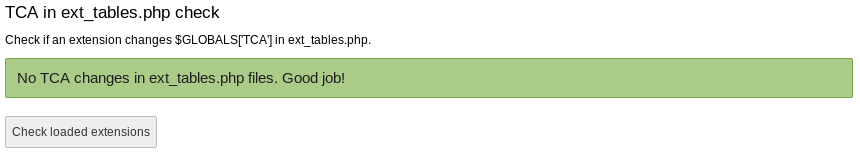
\includegraphics[width=0.95\linewidth]{DeprecatedRemovedFunctions/78384-install-tool-tca-in-exttables-check.png}
	\end{figure}

\end{frame}

% ------------------------------------------------------------------------------
% LTXE-SLIDE-START
% LTXE-SLIDE-UID:		3e8191ec-1c31f965-89f3f56d-76d8fb37
% LTXE-SLIDE-ORIGIN:	91358547-99cab1b1-208f0f24-a5737bee English
% LTXE-SLIDE-TITLE:		Removal of Fluid Styled Content Menu ViewHelpers (1/3)
% LTXE-SLIDE-REFERENCE:	!Breaking: #79622 - Removal of Fluid Styled Content Menu ViewHelpers
% ------------------------------------------------------------------------------

\begin{frame}[fragile]
	\frametitle{Extbase \& Fluid}
	\framesubtitle{Fluid Styled Content Menu ViewHelpers verwijderd (1/3)}

	\begin{itemize}
		\item Data direct ophalen in de 'view' is niet aan te raden en de tijdelijke oplossing
			van menu ViewHelpers is vervangen door de opvolger, de menu-processor
			gebaseerd op HMENU.

		\item Menu ViewHelpers zijn verplaatst naar de \texttt{compatibility7}
			extensie en vervangen in de core menu-inhoudselementen.

	\end{itemize}

\end{frame}

% ------------------------------------------------------------------------------
